\documentclass{article}
\usepackage{graphicx}
\usepackage{float}

\graphicspath{ {images/} }

\newcommand{\projectnaam}{Software Reengineering}
\newcommand{\student}{Van Muylder Ben \& Geeraert Lander}
\title{\textmd{\textbf{Final Project Report}}\\\normalsize\vspace{0.1in}\Large{\projectnaam}}
\author{\student}\date{\today}

\setcounter{section}{-1}

\begin{document}
\maketitle
\newpage

\section{Introduction}

The purpose of this project is to plan a refactoring for an existing software project such that we can easily add newly requested features.
The exiting software for this project is JFreeChart, and the functionality which we wish to add is the possibility to (1) have a plot where each data point is a different shape and (2) have the ability to read all different shapes from a database.\\

To be clear, we are not meant to implement these features, rather we are to refactor the project such that it would be easy for a developper to add these features.

\section{General Plan}

We will start by informing ourselves of the current structure and workings of this library. More specifically, we will figure out where and how exactly plots are generated in the code.\\

Using CodeScene, we looked at which classes it suggested needed refactoring (classes which were hotspots). This lead us to the XYPlot Class, which effectively is the class which renders plots.\\

XYPlot then uses a XYItemRenderer, or rather a class which implements the XYItemRenderer interface to effectively render its plots. Such a class could be XYLineAndShapeRenderer, which effectively renders a plot with shapes and lines which connects these shapes.\\

However, a XYLineAdnShapeRenderer is not capable of rendering a data set with all different shapes (which is were the assignment comes in place).\\

As such we can note that the ability for a serie of a plot to have a shape is already present it the code. This specific part is contained in the AbstractRenderer class. However, the class only allows you to set one specific shape for a serie. This is where we presume that our initial refactoring will take place.\\

For now we plan to split up the shape setting code/function to allow more flexible shape setting, for example: using multiple functions such as SetSeriesShapeUnique, SetSeriesShapeByType (where the type could be random)...

\begin{figure}[H]
\centering
	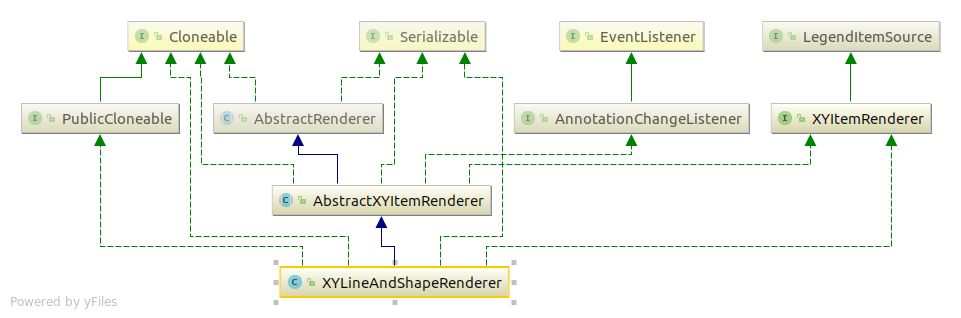
\includegraphics[width=0.9\textwidth]{XYLineAndShapeRenderer.png}
	\caption{an overview of the XYLineAndShapeRenderer and its dependencies}
\end{figure}

\section{The Refactoring Process}

\subsection{The first refactoring stage}

\subsubsection{Analysis}

As we discussed in the plan, we had found that the functionality which assigns the effective icon to a point on the plot resides in the AbstractRenderer class, more specifically in the function SetSeriesShape. We also discussed that we thought the initial refactor would be doen around this function. In this subsection, we'll discuss that refactor in further detail.\\

Let us first talk about what functionality this class, AbstractRenderer, already has concerning shapes. Among many other properties, the class has a defaultShape, a shapeList (which are both private properties) and a DEFAULT\_SHAPE (which is public, but only exists to set the initial value for the private defaultShape in the constructor of AbstractRenderer). There is also a property autoPopulateSeriesShape.\\

shapeList is a list which holds a shape for each serie from the renderer.
This means we can get 'get' (and 'set') the shape of each seperate serie. If the autoPopulateSeriesShape property should be true, and a series does not yet have an assigned shape, the 'get' function will try to assign a shape using a DrawingSupplier. We might further elaborate what this class is and does later on in the report, but it serves no further relevance here (as it supposed function seems clear from the class name). If the property autoPopulateSeriesShape should not be true, the serie shall remain without shape, but the default shape (defaultShape) will be returned.\\ 

From above mentioned behavior we can see that only a whole serie can have a shape (as opposed to single points from a serie). This is a logical choice, since we often generate series on plots not knowing how many points effectively will be generated, let alone that we would assign a different shape to those points. However, this current implementation does not allow for the requested behavior (as we have mentioned before).\\

Another general thing to note is that this class (AbstractRenderer) has a lot of functionality. We're not saying that this class is a god class, but we're also not saying that it's not a god class. Because of this it might be a good idea to consider splitting up some of the functionality of the class, particularly: the parts which are interesting for our case (functionality concerning shapes).

\subsubsection{Plan}

As we mentioned above, the AbstractRenderer class contains a lot of functionality, and that it might be a good plan to split up some of that functionality. That is what we plan to do to allow for the requested behaviour to be easily implemented. The plan is to take away the current functionality concerning shapes from the class, to put that functionality inside a separate class, which then will be used (or extended) by the AbstractRenderer class.\\ 

Having the original (and possibly slightly changed) functionality in a separate class, will allow future developpers to easily implement new features regarding the original functionality (in our case; shapes).

\begin{figure}[H]
\centering
	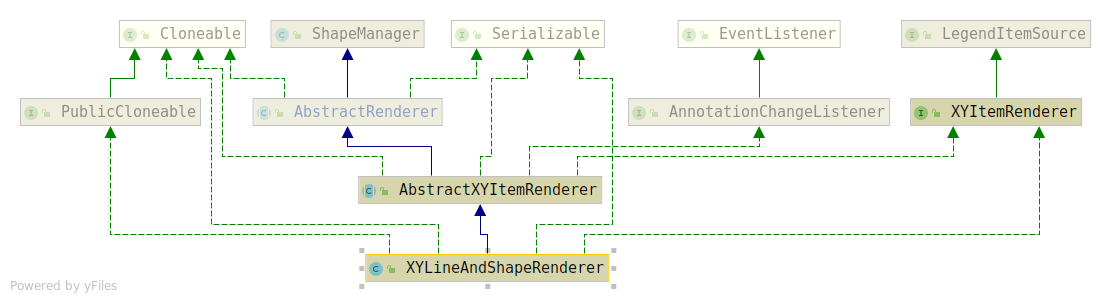
\includegraphics[width=0.9\textwidth]{RefactorStage1Design.png}
	\caption{an overview of the XYLineAndShapeRenderer and its dependencies, in respect to our proposed design change}
\end{figure}

\newpage
\section{Conclusion}


\end{document}